\documentclass{beamer}
\usepackage[utf8]{inputenc}

\usetheme{Madrid}
\usecolortheme{default}
\usepackage{amsmath,amssymb,amsfonts,amsthm}
\usepackage{txfonts}
\usepackage{tkz-euclide}
\usepackage{listings}
\usepackage{adjustbox}
\usepackage{array}
\usepackage{tabularx}
\usepackage{gvv}
\usepackage{lmodern}
\usepackage{circuitikz}
\usepackage{tikz}
\usepackage{graphicx}

\setbeamertemplate{page number in head/foot}[totalframenumber]

\usepackage{tcolorbox}
\tcbuselibrary{minted,breakable,xparse,skins}



\definecolor{bg}{gray}{0.95}
\DeclareTCBListing{mintedbox}{O{}m!O{}}{%
  breakable=true,
  listing engine=minted,
  listing only,
  minted language=#2,
  minted style=default,
  minted options={%
    linenos,
    gobble=0,
    breaklines=true,
    breakafter=,,
    fontsize=\small,
    numbersep=8pt,
    #1},
  boxsep=0pt,
  left skip=0pt,
  right skip=0pt,
  left=25pt,
  right=0pt,
  top=3pt,
  bottom=3pt,
  arc=5pt,
  leftrule=0pt,
  rightrule=0pt,
  bottomrule=2pt,
  toprule=2pt,
  colback=bg,
  colframe=orange!70,
  enhanced,
  overlay={%
    \begin{tcbclipinterior}
    \fill[orange!20!white] (frame.south west) rectangle ([xshift=20pt]frame.north west);
    \end{tcbclipinterior}},
  #3,
}
\lstset{
    language=C,
    basicstyle=\ttfamily\small,
    keywordstyle=\color{blue},
    stringstyle=\color{orange},
    commentstyle=\color{green!60!black},
    numbers=left,
    numberstyle=\tiny\color{gray},
    breaklines=true,
    showstringspaces=false,
}
%------------------------------------------------------------

\title
{12.705}
\date{October 11, 2025}
\author 
{AI25BTECH11003 - Bhavesh Gaikwad}



\begin{document}


\frame{\titlepage}
\begin{frame}{Question}
The minimum value of y for the equation $y = x^2 - 2x + 4$ is

\hfill{(MT 2021)}

\begin{itemize}
    \item[a)]3
    \item[b)]1
    \item[c)]4
    \item[d)]6
\end{itemize}

\end{frame}


\begin{frame}[fragile]
    \frametitle{Theoretical Solution}
Given:
\begin{equation}
 Parabola: \;   x^2 - 2x - y + 4 =0
\end{equation}

Parameters of the Parabola:
\begin{equation}
    \vec{V} = \myvec{1 & 0 \\ 0 & 0}, \quad \vec{u} = \myvec{-1 \\ -1/2}, \quad f = 4
\end{equation}

Equation of Parabola:
\begin{equation}
\vec{X}^\top\myvec{1 & 0 \\ 0 & 0}\vec{X} + 2\myvec{-1 & -1/2}\vec{X} + 4 = 0    
\end{equation}

Let line $L$ be parallel to the x-axis and passes through $y_{min}$.\\
Let $\phi$ represent the minimum value of $y$.
\begin{equation}
    \therefore \; L: \, \vec{X} = k\myvec{ 1 \\ 0} + \myvec{0 \\ \phi}
\end{equation}
\end{frame}

\begin{frame}[fragile]
\frametitle{Theoretical Solution}

Parameters of Line $L$:
\begin{equation}
\vec{m}= \myvec{1 \\ 0}, \quad \vec{h} = \myvec{0 \\ \phi}    
\end{equation}

Intersection of $L$ with Parabola:
\begin{equation}
    \vec{x}_i = k_i\vec{m} + \vec{h}
\end{equation}

\begin{equation}
    k_i = \dfrac{1}{\vec{m}^\top\vec{V}\vec{m}}\left( -\vec{m}^\top(\vec{V}\vec{h}+\vec{u})\pm \sqrt{[\vec{m}^\top(\vec{V}\vec{h}+\vec{u})]^2 - g(\vec{h})(\vec{m}^\top\vec{V}\vec{m})} \right)
\end{equation}
\end{frame}

\begin{frame}[fragile]
\frametitle{Theoretical Solution}
Since it is an opening upward parabola, therefore only one possible value of $y_{min}$ can occur.\\
Thus, only one value of $k$.
\begin{equation}
    \therefore \; [\vec{m}^\top(\vec{V}\vec{h}+\vec{u})]^2 - g(\vec{h})(\vec{m}^\top\vec{V}\vec{m}) = 0
\end{equation}

\begin{align}
    (-1)^2 - (4-\phi)(1) &= 0 \\
  \Rightarrow \, \boxed{\phi = 3}
\end{align}

\begin{align}
y_{min} = \phi = 3    
\end{align}

\begin{align*}
    \boxed{\text{Option-A is Correct.}}
\end{align*}
\end{frame}

\begin{frame}[fragile]
\frametitle{Image}
\begin{figure}
   \centering
    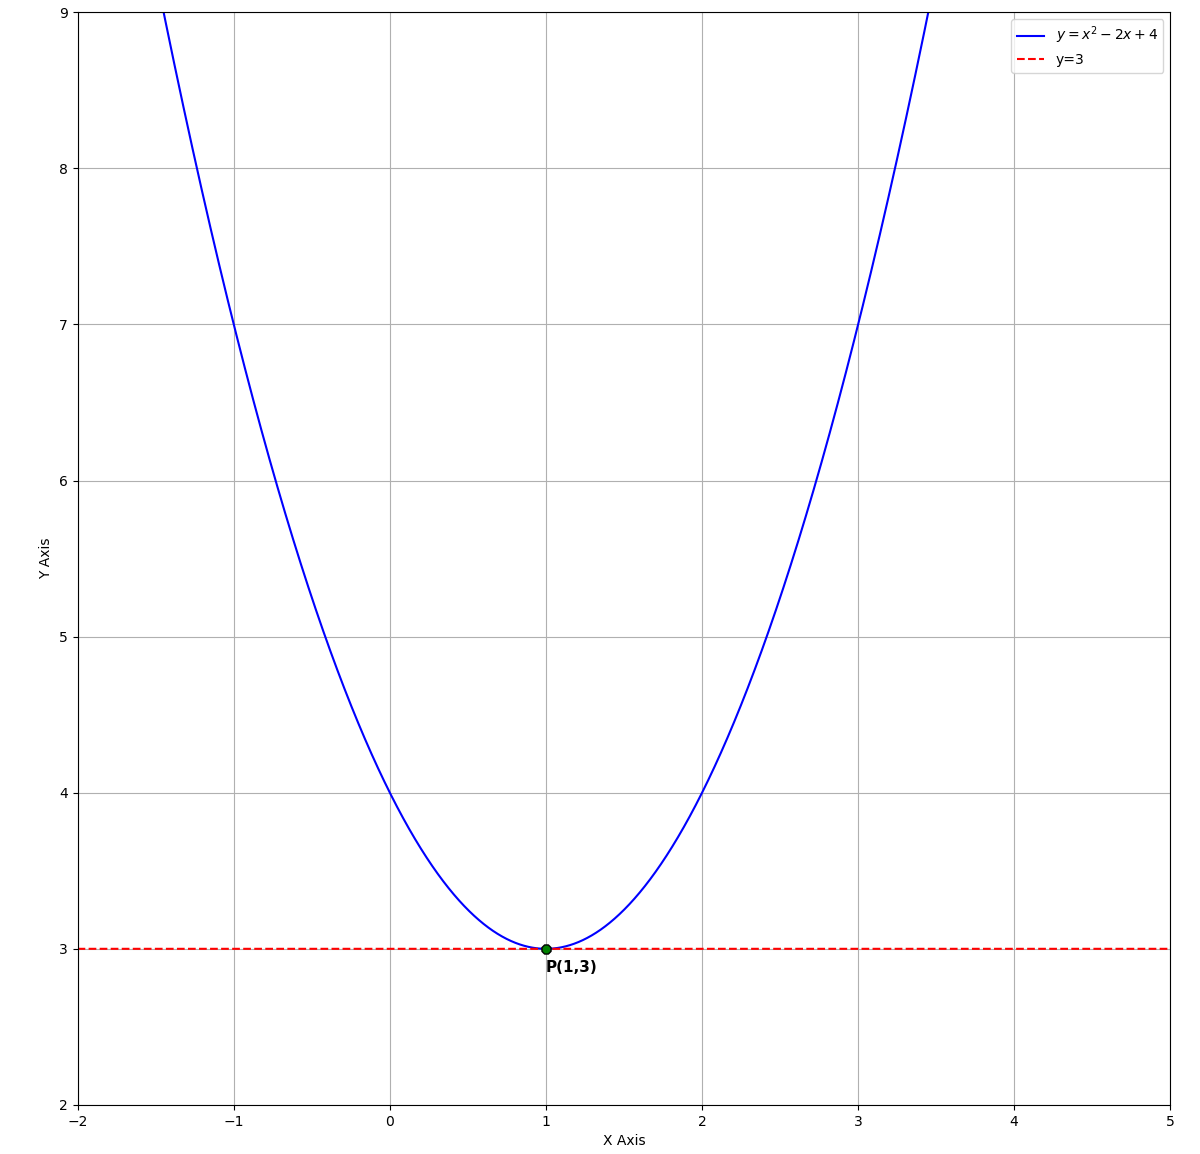
\includegraphics[width=\columnwidth, height=0.8\textheight, keepaspectratio]{figs/fig1.png}
    \label{fig:Beamer/figs/fig1.png}
\end{figure}
\end{frame}


\end{document}